\vspace{-0.5em}
\section{Introduction}
Materialized views (MVs), stored pre-computed results, are a well-studied approach to speed up queries on large datasets \cite{LarsonY85, gupta1995maintenance, chirkova2011materialized, halevy2001answering}.
During the last 30 years, the research community has thoroughly studied MVs, and all major database vendors have added support for them for traditional query processing and recently for more advanced analytics based on linear algebra and machine learning \cite{nikolic2014linview, zhang2014mat}.

However, when the underlying data is changed MVs can become \emph{stale}; the pre-computed results do not reflect the recent changes to the data. 
One solution would be to recompute the MV every time a change occurs; however, in many cases, it is more efficient to incrementally update the MV instead of recomputation.
There has been substantial work in deriving incremental updates (incremental maintenance) for different classes of MVs and optimizing their execution \cite{chirkova2011materialized}.

For frequently changing tables even incremental maintenance can be expensive since every update to the base data requires updating all the dependent views.  
In many important applications, such as summary statistics from server logs, new records arrive at a fast rate and data are often distributed across multiple machines making incremental maintenance infeasible. 
As a result, in production environments, it is common to defer view maintenance \cite{chirkova2011materialized, zhou2007lazy, DBLP:conf/sigmod/ColbyGLMT96} so that updates can be batched together to amortize overheads and can be scheduled at times of low system utilization (e.g., nightly).  

While deferring maintenance has benefits, the views are stale in between maintenance periods.
As a result, as the time since the last maintenance increases, queries on those views can return incorrect answers.
The problem of stale MVs parallels the problem of dirty data studied in data cleaning~\cite{rahm2000data}.
As in the data cleaning, a stale MV leads to incorrect, missing, or superfluous rows.
In this paper, we explore how answering queries on a stale MV can be formalized as a data cleaning problem. 
%This observation leads us to the main insight behind our work; namely, that a data cleaning approach can be applied to mitigate the negative impacts of deferred MV maintenance.

\begin{figure}[t] \vspace{-2em}
\centering
 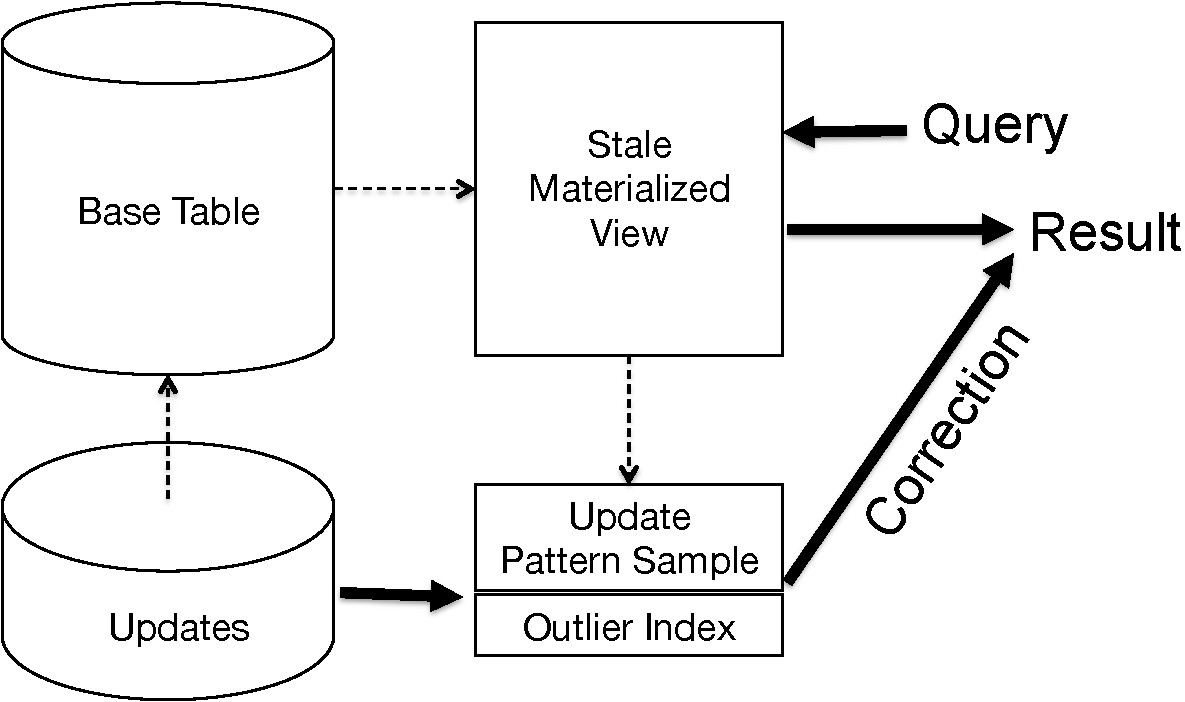
\includegraphics[scale=0.25]{figs/sys-arch.pdf} \vspace{-.25em}
 \caption{Deferred maintenance can lead to stale MVs which have incorrect, missing, and superflous rows. In \svc, we pose this as a data cleaning problem and show that we can use a sample of clean (up-to-date) rows from an MV to correct inaccurate query results on the stale view. We also devise an outlier indexing technique for more accurate corrections in skewed datasets. \label{sys-arch}}\vspace{-1.75em}
\end{figure}

Data cleaning has been studied extensively in the literature (e.g., see Rahm and Do for a survey\cite{rahm2000data}) but increasing data volumes and arrival rates have led to development of new, efficient sampling-based approaches for coping with dirty data.   
In our prior work, we developed the SampleClean framework for scalable aggregate query processing on dirty data \cite{wang1999sample}.
If we have an expensive data cleaning operation, we can apply the cleaning to a sample of data and use this sample to improve the results of aggregate queries.
This perspective raises a new possibility for MVs: we can use a sample of clean (up-to-date) rows in the MV to return more accurate query results only incurring the cost of maintaining a sample of the MV.
In this paper, we propose \svcfull (SVC), which uses sampling for less expensive query processing on stale materialized views.

%We treated data cleaning as a ``black-box" and applied it to a sample of data and used this clean sample to improve the results of aggregate queries.

SVC takes a sample of up-to-date rows from the view, analyzes how those rows changed from the stale MV, and extrapolates a correction factor for query answers on the stale view. Figure~\ref{sys-arch} shows how \svc can be used as complementary to existing deferred maintenance approaches. 
When the MVs become stale between maintenance cycles, we apply \svc for query result estimation for a far smaller cost than having to maintain the entire view.
The query results from \svc are up-to-date in the sense that they reflect the most recent data, however they are approximate. 
The approximation error due to sampling is more manageable than staleness because: (1) the uniformity of sampling allows us to apply theory from statistics such as the Central Limit Theorem to give tight bounds on approximate results, and (2) the approximate error is parameterized by the sample size which the user can control trading off accuracy for computation.
Sampling is known to be sensitive to skewed datasets, and we incorporate an outlier indexing technique to improve the accuracy of our approximation.
A significant challenge is efficiently computing this index in a single pass of the base data and deciding when we can use the outlier index to improve our estimates.


%Both MVs and queries can be complex.
Since \svc is based on sampling, there are a subclass of views for which \svc can save significant computation and a subclass of queries on these views for which \svc can give accurate corrections.
In this work, we explore these classes from both a theoretical perspective (i.e., when is our query correction optimal w.r.t estimate variance) and an empirical perspective for queries that do not satisfy the optimality conditions when is \svc still beneficial.

To summarize, our contributions are as follows: (1) we formalize maintenance of a sample MV as a data cleaning operation allowing us to apply sample-based clean aggregate query processing, (2) we devise an query processing approach to answer queries accurately using the sample of up-to-date data, (3) we use an outlier index to increase the accuracy of the approach for power-law, long-tailed, and skewed distributions, and (4) we evaluate our approach on real and synthetic datasets confirming that indeed sampling can reduce view maintenance time while providing accurate query results. 
%\end{itemize}

The paper is organized as follows: 
In Section~\ref{sec-background}, we give the necessary background for our work.
Next, in Section~\ref{sec-arch}, we formalize the problem.
In Sections~\ref{sampling} and~\ref{correction}, we describe the sampling and query processing of our technique.
In Section~\ref{outlier}, we describe the outlier indexing framework.
%In Section~\ref{sec:ext}, we discuss extensions to our framework.
Then, in Section~\ref{exp}, we evaluate our approach.
Finally, we discuss Related Work in Section~\ref{related} and present our Conclusions and Future Work in Section~\ref{conclusion}.
We present full versions of our proofs and experimental details in our extended technical report \cite{technicalReport}.
